%%%%%%%%%%%%%%%%%%%%%%%%%%%%%%%%%%%%%%%%%
% a0poster Portrait Poster
% LaTeX Template
% Version 1.0 (22/06/13)
%
% The a0poster class was created by:
% Gerlinde Kettl and Matthias Weiser (tex@kettl.de)
% 
% This template has been downloaded from:
% http://www.LaTeXTemplates.com
%
% License:
% CC BY-NC-SA 3.0 (http://creativecommons.org/licenses/by-nc-sa/3.0/)
%
%%%%%%%%%%%%%%%%%%%%%%%%%%%%%%%%%%%%%%%%%

%HIGH:
%TIMEBOX!!
%TODO primero pasar a git
%TODO achicar imágenes (poner en dos columnas)
%TODO llenar con más información 
%TODO referencias

%LOW:
%TODO mover logo departamento

%----------------------------------------------------------------------------------------
%	PACKAGES AND OTHER DOCUMENT CONFIGURATIONS
%----------------------------------------------------------------------------------------

\documentclass[a0,portrait]{a0poster}

\usepackage{multicol} % This is so we can have multiple columns of text side-by-side
\columnsep=100pt % This is the amount of white space between the columns in the poster
\columnseprule=3pt % This is the thickness of the black line between the columns in the poster

\usepackage[svgnames]{xcolor} % Specify colors by their 'svgnames', for a full list of all colors available see here: http://www.latextemplates.com/svgnames-colors

\usepackage{times} % Use the times font
%\usepackage{palatino} % Uncomment to use the Palatino font

\usepackage{graphicx} % Required for including images
\graphicspath{{figures/}} % Location of the graphics files
\usepackage{booktabs} % Top and bottom rules for table
\usepackage[font=small,labelfont=bf]{caption} % Required for specifying captions to tables and figures
\usepackage{amsfonts, amsmath, amsthm, amssymb} % For math fonts, symbols and environments
\usepackage{wrapfig} % Allows wrapping text around tables and figures

\usepackage[utf8x]{inputenc}			%acentos, etc
\usepackage[spanish,activeacute]{babel}	%titulos en castellano
\usepackage[version=3]{mhchem}			%química
\usepackage{siunitx}					%unidades

\begin{document}

\newcommand{\h}{\ce{H^+}}
\newcommand{\oh}{\ce{OH^-}}
\newcommand{\na}{\ce{Na^+}}
\newcommand{\cl}{\ce{Cl^-}}
\newcommand{\kvm}{$\si{\kilo\volt\per\metre}$}
\newcommand{\usec}{$\si{\micro\second}$}

%----------------------------------------------------------------------------------------
%	POSTER HEADER 
%----------------------------------------------------------------------------------------

% The header is divided into two boxes:
% The first is 75% wide and houses the title, subtitle, names, university/organization and contact information
% The second is 25% wide and houses a logo for your university/organization or a photo of you
% The widths of these boxes can be easily edited to accommodate your content as you see fit

\begin{minipage}[b]{0.75\linewidth}
\veryHuge \color{NavyBlue} \textbf{Modelado de Electroporación Celular} \color{Black}\\ % Title
%\Huge\textit{An Exploration of Complexity}\\[2cm] % Subtitle PUEDE IR UN SUBTITULO
%\huge \textbf{John Smith \& James Smith}\\[0.5cm] % Author(s)
%\huge University and Department Name\\[0.4cm] % University/organization
%\Large \texttt{john@LaTeXTemplates.com} --- 1 (000) 111 1111\\

\huge \textbf{Mauricio Alfonso} - LSC, FCEyN\\[0.5cm]
\huge \textbf{Alejandro Soba} - CSC-CONICET\\[0.5cm]
\huge \textbf{Guillermo Marshall} - INFIP, CONICET\\[0.5cm]

\end{minipage}
%
\begin{minipage}[b]{0.25\linewidth}

\includegraphics[width=20cm]{logodc.jpg}\\
\end{minipage}

\vspace{1cm} % A bit of extra whitespace between the header and poster content

%----------------------------------------------------------------------------------------

\begin{multicols}{2} % This is how many columns your poster will be broken into, a portrait poster is generally split into 2 columns

\color{Navy} % Navy color for the abstract

%\begin{abstract}
%\large
\begin{center}Introducción\end{center}
La electroporación reversible es un método consistente en la aplicación de pulsos eléctricos de alta intensidad a una célula con el objetivo de permeabilizar su membrana creando poros, y así permitir el ingreso de drogas o moléculas de ADN a su interior. Esto permite tratar tumores con menores cantidades de drogas, reduciendo los efectos secundarios.\\

En este trabajo se simula una célula esférica a la que se le aplica un pulso eléctrico de 20\si{\milli\second} de duración a través de dos electrodos, y se estudia el ingreso al interior de la célula de 4 especies iónicas: el ión hidrógeno (\h), el hidróxido (\oh), el catión sodio (\na) y el cloruro (\cl). Para eso se tiene en cuenta el campo eléctrico producido por los electrodos, la generación y evolución de poros en la membrana celular producto de la diferencia de potencial entre el interior y exterior de la célula , y la migración de las especies mencionadas, producto de la diferencia de potencial.\\

Las simulaciones se realizaron con el método de elementos finitos sobre mallas bidimensionales que representan el dominio sobre un sistema de coordenadas cilíndricas usando elementos cuadrilaterales.

%\end{abstract}

%\color{SaddleBrown} % SaddleBrown color for the introduction

%\section*{Introduction}
%
%Aliquam non lacus dolor, \textit{a aliquam quam} \cite{Smith:2012qr}. Cum sociis natoque penatibus et magnis dis parturient montes, nascetur ridiculus mus. Nulla in nibh mauris. Donec vel ligula nisi, a lacinia arcu. Sed mi dui, malesuada vel consectetur et, egestas porta nisi. Sed eleifend pharetra dolor, et dapibus est vulputate eu. \textbf{Integer faucibus elementum felis vitae fringilla.} In hac habitasse platea dictumst. Duis tristique rutrum nisl, nec vulputate elit porta ut. Donec sodales sollicitudin turpis sed convallis. Etiam mauris ligula, blandit adipiscing condimentum eu, dapibus pellentesque risus.
%
%\textit{Aliquam auctor}, metus id ultrices porta, risus enim cursus sapien, quis iaculis sapien tortor sed odio. Mauris ante orci, euismod vitae tincidunt eu, porta ut neque. Aenean sapien est, viverra vel lacinia nec, venenatis eu nulla. Maecenas ut nunc nibh, et tempus libero. Aenean vitae risus ante. Pellentesque condimentum dui. Etiam sagittis purus non tellus tempor volutpat. Donec et dui non massa tristique adipiscing.

\color{DarkSlateGray} % DarkSlateGray color for the rest of the content

\section*{Teoría}

%\subsection*{Potencial Eléctrico}
Potencial eléctrico
			\begin{equation}
				\sigma_{e} \nabla^2 \phi = 0
			\end{equation}

%			Con $\phi$ el potencial eléctrico y $\sigma_{e}$ la conductividad del material.
%			Condiciones de borde de Dirichlet en los electrodos y Neumann en los otros bordes.\\
			
%			El potencial transmembrana (ITV) debería aproximarse a:
%			\begin{center}
%				$V^{\theta} = 1.5 E cos (\theta)$
%			\end{center}

			Se asume que la membrana se carga como un capacitor en paralelo con una resistencia:
			\begin{equation}
				V_m = V_p (1 - e^{-t/\tau}),
			\end{equation}
			\begin{equation}
				\textrm{con } \tau = \alpha C_m \left( \frac{1}{\sigma_i} + \frac{1}{2 \sigma_o} \right)
			\end{equation}\\
			
%			Con $\alpha$ el radio, $C_m$ la capacitancia de la membrana y $\sigma_i$ y $\sigma_o$ las
%			conductividades interna y externa.

	Densidad de poros:
	\begin{equation}
		\frac{\partial N}{\partial t} = \alpha_c e^{(V_m/V_{ep})^2} 
			\left( 1 - \frac{N}{N_0 e^{q \left(V_m/V_{ep} \right) ^2}} \right)
	\end{equation}
	La densidad depende del ITV en cada región de la célula 
	(no es constante en toda la superficie).\\
%	\newline 
	%			$N$ es la densidad de poros, $V_m$ es el ITV, $\alpha_c$ es el coeficiente de creación de poros, 
	%			$V_{ep}$ es el voltaje característico de electroporación, 
	%			$N_0$ es la densidad de poros en equilibrio (cuando $V_m = 0$) y 
	%			$q$ es una constante igual a $(r_m / r*)^2$, donde $r_m$ es el radio de mínima energía 
	%			para $V_m = 0$ y $r*$ es el radio mínimo de los poros.\\

%	$N$ es la densidad de poros, $V_m$ es el ITV, 
%	$\alpha_c$, $V_{ep}$, $N_0$ y $q$ constantes.

	Radio de los poros:
	\begin{equation}
		\frac{\partial r}{\partial t} = \frac{D}{kT} \left( \frac{V_m^2 F_{max}}
			{1+r_h / (r+r_a)} + \frac{4 \beta}{r} \left(\frac{r_*}{r}\right)^4 
			- 2 \pi \gamma + 2 \pi \sigma_{\textrm{\tiny eff}} r\right), 
	\end{equation}

	\begin{equation}
		\textrm{con }\sigma_{\textrm{\tiny eff}} = 2 \sigma^\prime - 
			\frac{2 \sigma^\prime - \sigma_0}{(1 - A_p / A)^2}
	\end{equation}	\\
	

	%			\begin{center}
	%				$ \textrm{con } \sigma_{\textrm{\tiny eff}} = 2 \sigma^\prime - 
	%					\frac{2 \sigma^\prime - \sigma_0}{(1 - A_p / A)^2}	$
	%			\end{center}

	Se aplica a cada poro por separado.\\


	Transporte de especies: ecuación de Nernst-Planck
	\begin{equation}
		\frac{\partial C_i}{\partial t} = \nabla \cdot \left( D_i \nabla C_i + D_i z_i 
			\frac{F}{R T} C_i \nabla \phi \right)
	\end{equation}	\\			
%	donde $C_i$, $D_i$ y $z_i$ son la concentración, la difusión y la valencia de la 
%		especie $i$, para $i$ alguna de las especies mencionadas (\h, \oh, \na, \cl).
%	\newline \newline		
%	$F$ y $R$ son las constantes de Faraday y de los gases y $T$ la temperatura.

	La conductividad de la membrana se recalcula según el área ocupada por los poros		
	\begin{equation}
		\sigma_{e} = \sigma_m (1 - p) + \sigma_p p
	\end{equation}\\
%	donde $p$ es la proporción ocupada por poros de una zona esférica de la membrana. 
%	$\sigma_m$ y $\sigma_p$ son las conductividades de la membrana sin poros y del líquido 
%	que llena el poro
%	\newline \newline
	Lo mismo se hace con la difusión:
	\begin{equation}
		D_{i, e} = D_i (1 - p) + D_p
	\end{equation}

%	D_m$ y $D_p$ son las conductividades de la membrana sin poros y del líquido 
%	que llena el poro


\section*{Resultados}

%\begin{center}\vspace{1cm}
%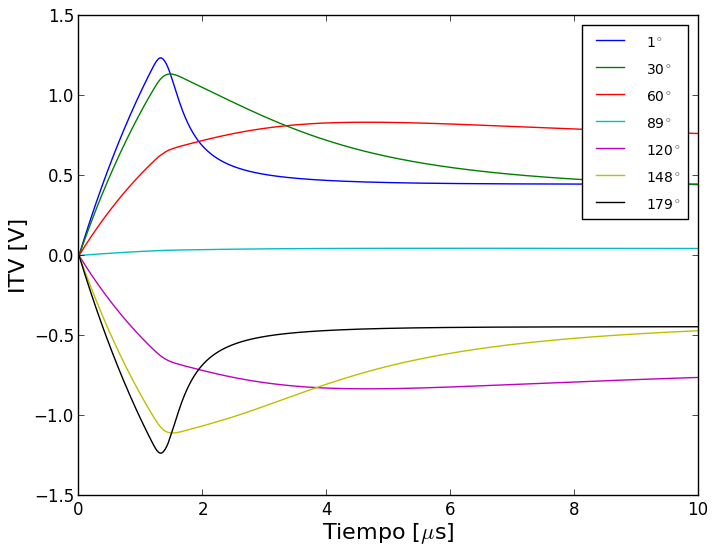
\includegraphics[width=0.8\linewidth]{itv-time-lin-25-64-80KVm}
%\captionof{figure}{\color{Green} ITV vs. tiempo para distintos ángulos para $\alpha$ = 25\si{\micro\metre} y 40\kvm}
%\end{center}\vspace{1cm}

\begin{center}\vspace{1cm}
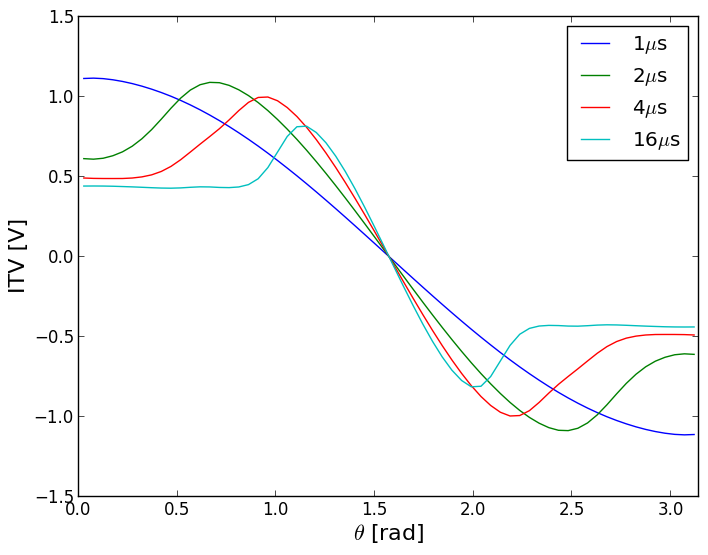
\includegraphics[width=0.8\linewidth]{itv-tita-50-64-80KVm}
\captionof{figure}{\color{Green} ITV vs. ángulo en distintos instantes para $\alpha$ = 25\si{\micro\metre} y 40\kvm}
\end{center}\vspace{1cm}

\begin{center}\vspace{1cm}
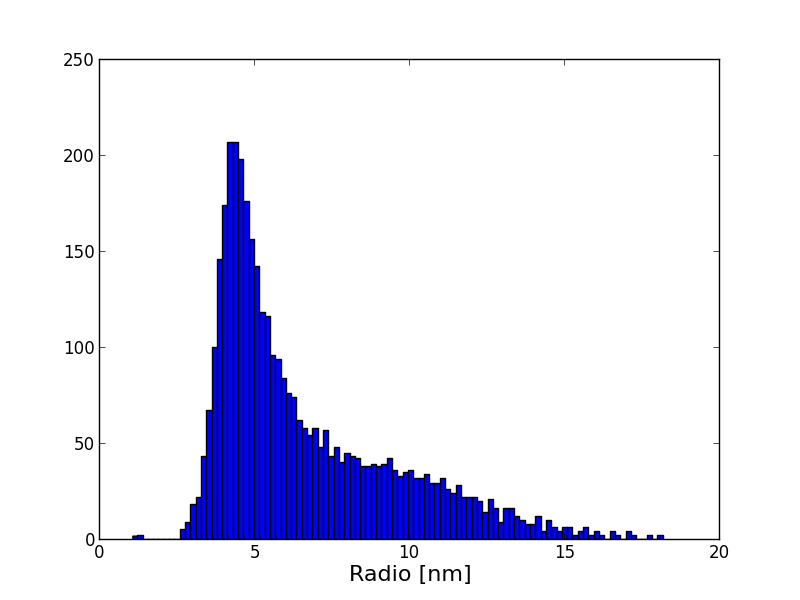
\includegraphics[width=0.8\linewidth]{hist-radios-5e-6-50-64-120KVm}
\captionof{figure}{\color{Green} Distribución de poros para $\alpha$ = 50\si{\micro\metre}, 120\kvm en t = 5 \usec}
\end{center}\vspace{1cm}

\section*{Conclusiones}
			\begin{itemize}
				\item Se pueden ingresar las especies, pero se necesitan voltajes muy altos,
					sobre todo para \na y \cl
				\item Los poros generados disminuyen la conductancia de la membrana, 
					disminuyendo el ITV
				\item El voltaje aplicado influye en la velocidad con la que se crean los poros,
					pero no aumenta el ITV, siempre que se alcance un valor mínimo
				\item La mayoría de los poros creados se cierran muy rápidamente; antes de que 
					lleguen las especies, luego no sirven para permeabilizar la membrana
			\end{itemize}



%%----------------------------------------------------------------------------------------
%%	OBJECTIVES
%%----------------------------------------------------------------------------------------
%
%
%
%\section*{Main Objectives}
%
%\begin{enumerate}
%\item Lorem ipsum dolor sit amet, consectetur.
%\item Nullam at mi nisl. Vestibulum est purus, ultricies cursus volutpat sit amet, vestibulum eu.
%\item Praesent tortor libero, vulputate quis elementum a, iaculis.
%\item Phasellus a quam mauris, non varius mauris. Fusce tristique, enim tempor varius porta, elit purus commodo velit, pretium mattis ligula nisl nec ante.
%\item Ut adipiscing accumsan sapien, sit amet pretium.
%\item Estibulum est purus, ultricies cursus volutpat
%\item Nullam at mi nisl. Vestibulum est purus, ultricies cursus volutpat sit amet, vestibulum eu.
%\item Praesent tortor libero, vulputate quis elementum a, iaculis.
%\end{enumerate}
%
%%----------------------------------------------------------------------------------------
%%	MATERIALS AND METHODS
%%----------------------------------------------------------------------------------------
%
%\section*{Materials and Methods}
%
%Fusce magna risus, molestie ut porttitor in, consectetur sed mi. Vestibulum ante ipsum primis in faucibus orci luctus et ultrices posuere cubilia Curae; Pellentesque consectetur blandit pellentesque. Sed odio justo, viverra nec porttitor vel, lacinia a nunc. Suspendisse pulvinar euismod arcu, sit amet accumsan enim fermentum quis. In id mauris ut dui feugiat egestas. Vestibulum ac turpis lacinia nisl commodo sagittis eget sit amet sapien.
%
%%------------------------------------------------
%
%\subsection*{Mathematical Section}
%
%Nulla vel nisl sed mauris auctor mollis non sed. 
%
%\begin{equation}
%E = mc^{2}
%\label{eqn:Einstein}
%\end{equation}
%
%Curabitur mi sem, pulvinar quis aliquam rutrum. (1) edf (2)
%, $\Omega=[-1,1]^3$, maecenas leo est, ornare at. $z=-1$ edf $z=1$ sed interdum felis dapibus sem. $x$ set $y$ ytruem. 
%Turpis $j$ amet accumsan enim $y$-lacina; 
%ref $k$-viverra nec porttitor $x$-lacina. 
%
%Vestibulum ac diam a odio tempus congue. Vivamus id enim nisi:
%
%\begin{eqnarray}
%\cos\bar{\phi}_k Q_{j,k+1,t} + Q_{j,k+1,x}+\frac{\sin^2\bar{\phi}_k}{T\cos\bar{\phi}_k} Q_{j,k+1} &=&\nonumber\\ 
%-\cos\phi_k Q_{j,k,t} + Q_{j,k,x}-\frac{\sin^2\phi_k}{T\cos\phi_k} Q_{j,k}\label{edgek}
%\end{eqnarray}
%and
%\begin{eqnarray}
%\cos\bar{\phi}_j Q_{j+1,k,t} + Q_{j+1,k,y}+\frac{\sin^2\bar{\phi}_j}{T\cos\bar{\phi}_j} Q_{j+1,k}&=&\nonumber \\
%-\cos\phi_j Q_{j,k,t} + Q_{j,k,y}-\frac{\sin^2\phi_j}{T\cos\phi_j} Q_{j,k}.\label{edgej}
%\end{eqnarray} 
%
%Nulla sed arcu arcu. Duis et ante gravida orci venenatis tincidunt. Fusce vitae lacinia metus. Pellentesque habitant morbi. $\mathbf{A}\underline{\xi}=\underline{\beta}$ Vim $\underline{\xi}$ enum nidi $3(P+2)^{2}$ lacina. Id feugain $\mathbf{A}$ nun quis; magno.

%%----------------------------------------------------------------------------------------
%%	RESULTS 
%%----------------------------------------------------------------------------------------
%
%\section*{Results}
%
%Donec faucibus purus at tortor egestas eu fermentum dolor facilisis. Maecenas tempor dui eu neque fringilla rutrum. Mauris \emph{lobortis} nisl accumsan. Aenean vitae risus ante.
%%
%\begin{wraptable}{l}{12cm} % Left or right alignment is specified in the first bracket, the width of the table is in the second
%\begin{tabular}{l l l}
%\toprule
%\textbf{Treatments} & \textbf{Response 1} & \textbf{Response 2}\\
%\midrule
%Treatment 1 & 0.0003262 & 0.562 \\
%Treatment 2 & 0.0015681 & 0.910 \\
%Treatment 3 & 0.0009271 & 0.296 \\
%\bottomrule
%\end{tabular}
%\captionof{table}{\color{Green} Table caption}
%\end{wraptable}
%%
%Phasellus imperdiet, tortor vitae congue bibendum, felis enim sagittis lorem, et volutpat ante orci sagittis mi. Morbi rutrum laoreet semper. Morbi accumsan enim nec tortor consectetur non commodo nisi sollicitudin. Proin sollicitudin. Pellentesque eget orci eros. Fusce ultricies, tellus et pellentesque fringilla, ante massa luctus libero, quis tristique purus urna nec nibh.
%
%Nulla ut porttitor enim. Suspendisse venenatis dui eget eros gravida tempor. Mauris feugiat elit et augue placerat ultrices. Morbi accumsan enim nec tortor consectetur non commodo. Pellentesque condimentum dui. Etiam sagittis purus non tellus tempor volutpat. Donec et dui non massa tristique adipiscing. Quisque vestibulum eros eu. Phasellus imperdiet, tortor vitae congue bibendum, felis enim sagittis lorem, et volutpat ante orci sagittis mi. Morbi rutrum laoreet semper. Morbi accumsan enim nec tortor consectetur non commodo nisi sollicitudin.
%
%\begin{center}\vspace{1cm}
%
\includegraphics[width=0.8\linewidth]{placeholder}
%\captionof{figure}{\color{Green} Figure caption}
%\end{center}\vspace{1cm}
%
%In hac habitasse platea dictumst. Etiam placerat, risus ac.
%
%Adipiscing lectus in magna blandit:
%
%\begin{center}\vspace{1cm}
%\begin{tabular}{l l l l}
%\toprule
%\textbf{Treatments} & \textbf{Response 1} & \textbf{Response 2} \\
%\midrule
%Treatment 1 & 0.0003262 & 0.562 \\
%Treatment 2 & 0.0015681 & 0.910 \\
%Treatment 3 & 0.0009271 & 0.296 \\
%\bottomrule
%\end{tabular}
%\captionof{table}{\color{Green} Table caption}
%\end{center}\vspace{1cm}
%
%Vivamus sed nibh ac metus tristique tristique a vitae ante. Sed lobortis mi ut arcu fringilla et adipiscing ligula rutrum. Aenean turpis velit, placerat eget tincidunt nec, ornare in nisl. In placerat.
%
%\begin{center}\vspace{1cm}
%
\includegraphics[width=0.8\linewidth]{placeholder}
%\captionof{figure}{\color{Green} Figure caption}
%\end{center}\vspace{1cm}
%
%%----------------------------------------------------------------------------------------
%%	CONCLUSIONS
%%----------------------------------------------------------------------------------------
%
%\color{SaddleBrown} % SaddleBrown color for the conclusions to make them stand out
%
%\section*{Conclusions}
%
%\begin{itemize}
%\item Pellentesque eget orci eros. Fusce ultricies, tellus et pellentesque fringilla, ante massa luctus libero, quis tristique purus urna nec nibh. Phasellus fermentum rutrum elementum. Nam quis justo lectus.
%\item Vestibulum sem ante, hendrerit a gravida ac, blandit quis magna.
%\item Donec sem metus, facilisis at condimentum eget, vehicula ut massa. Morbi consequat, diam sed convallis tincidunt, arcu nunc.
%\item Nunc at convallis urna. isus ante. Pellentesque condimentum dui. Etiam sagittis purus non tellus tempor volutpat. Donec et dui non massa tristique adipiscing.
%\end{itemize}
%
%\color{DarkSlateGray} % Set the color back to DarkSlateGray for the rest of the content
%
%%----------------------------------------------------------------------------------------
%%	FORTHCOMING RESEARCH
%%----------------------------------------------------------------------------------------
%
%\section*{Forthcoming Research}
%
%Vivamus molestie, risus tempor vehicula mattis, libero arcu volutpat purus, sed blandit sem nibh eget turpis. Maecenas rutrum dui blandit lorem vulputate gravida. Praesent venenatis mi vel lorem tempor at varius diam sagittis. Nam eu leo id turpis interdum luctus a sed augue. Nam tellus.
%
% %----------------------------------------------------------------------------------------
%%	REFERENCES
%%----------------------------------------------------------------------------------------
%
%\nocite{*} % Print all references regardless of whether they were cited in the poster or not
%\bibliographystyle{plain} % Plain referencing style
%\bibliography{sample} % Use the example bibliography file sample.bib
%
%%----------------------------------------------------------------------------------------
%%	ACKNOWLEDGEMENTS
%%----------------------------------------------------------------------------------------
%
%\section*{Acknowledgements}
%
%Etiam fermentum, arcu ut gravida fringilla, dolor arcu laoreet justo, ut imperdiet urna arcu a arcu. Donec nec ante a dui tempus consectetur. Cras nisi turpis, dapibus sit amet mattis sed, laoreet.
%
%%----------------------------------------------------------------------------------------

\end{multicols}
\end{document}